\documentclass[a4paper,10pt]{article}
\usepackage[utf8]{inputenc}
\usepackage[english]{babel}
\usepackage{indentfirst}
\usepackage{geometry}
\usepackage{fancyhdr} % For custom headers
\usepackage{lastpage} % To determine the last page for the footer
\usepackage{extramarks} % For headers and footers
%\usepackage[most]{tcolorbox} % For problem answer sections
\usepackage{graphicx,subfigure} % For inserting images
\usepackage{color,soul} % For link coloring
\usepackage[hidelinks]{hyperref} % For URL links (no box or color name)
\usepackage{csquotes}
\usepackage[labelfont=bf]{caption}
\usepackage{textcomp}
\usepackage{enumitem}
\usepackage{fourier}
\usepackage{listings}


\definecolor{mygreen}{RGB}{28,172,0} % color values Red, Green, Blue
\definecolor{mylilas}{RGB}{170,55,241}


% Margins
\geometry{
a4paper,
tmargin=1in,
bmargin=1in,
lmargin=1in,
rmargin=1in,
textwidth=6.5in,
textheight=9.0in,
headsep=0.25in
}

% Header and footer
\pagestyle{fancy}
\lhead{SCERPA documentation} % Top left header
\chead{} % Top center header
\rhead{VLSI Lab\firstxmark} % Top right header
\lfoot{\myDueDate} % Bottom left footer
\cfoot{} % Bottom center footer
\rfoot{Page\ \thepage\ of\ \pageref{LastPage}} % Bottom right footer
\renewcommand\headrulewidth{0.4pt} % Size of the header rule
\renewcommand\footrulewidth{0.4pt} % Size of the footer rule

% Other configurations
\setlength\parindent{0pt} % Removes all indentation from paragraphs
\setlength\parskip{1pt} % Ensures paragraphs are still recognizable as such
%\setcounter{secnumdepth}{0} % Removes default section numbers
\setcounter{tocdepth}{3} % Sets depth of table of contents
\linespread{1.1}

% Template values
\newcommand{\myFirstLogo}{vlsilogoNanocomp.png}
\newcommand{\mySecondLogo}{Polito_Logo_2021_BLU.png}
\newcommand{\myName}{Giuliana Beretta}
\newcommand{\myEmail}{giuliana.beretta@polito.it}
\newcommand{\myColleagueName}{Yuri Ardesi}
\newcommand{\myColleagueEmail}{yuri.ardesi@polito.it}
\newcommand{\myTitle}{SCERPA documentation}
\newcommand{\VLSItitle}{VLSI Lab - Politecnico di Torino}
\newcommand{\VLSIdep}{Department of Electronics and Telecommunications}
\newcommand{\VLSIurl}{https://www.vlsilab.polito.it/}
\newcommand{\authorTitle}{Authors}
\newcommand{\myDueDate}{June 2020}

%----------------------------------------------------------------------------------------
%  DOCUMENT STRUCTURE (MACROS & ENVIRONMENTS)
%----------------------------------------------------------------------------------------

% Colored links macro
%\newcommand{\hrefcol}[3] {\href{#1}{\textcolor{#3}{#2}}}
\setlength\parindent{24pt}

% Macro for custom title page signature header
\newsavebox{\myLogos}
\sbox{\myLogos}{%
\begin{tabular*}{\textwidth}{@{}l@{}r@{\extracolsep{0.125in}}l@{}}%
\parbox{9cm}{\raggedright{\includegraphics[width=3.5cm]{\myFirstLogo}}} &
\parbox{9cm}{\raggedright{\includegraphics[width=5cm]{\mySecondLogo}}}
\end{tabular*}}


\begin{document}
%\lstset{language=Matlab,%
%    %basicstyle=\color{red},
%    breaklines=true,%
%    morekeywords={matlab2tikz},
%    keywordstyle=\color{blue},%
%    morekeywords=[2]{1}, keywordstyle=[2]{\color{black}},
%    identifierstyle=\color{black},%
%    stringstyle=\color{mylilas},
%    commentstyle=\color{mygreen},%
%    showstringspaces=false,%without this there will be a symbol in the places where there is a space
%    numbers=left,%
%    numberstyle={\tiny \color{black}},% size of the numbers
%    numbersep=9pt, % this defines how far the numbers are from the text
%    emph=[1]{for,end,break},emphstyle=[1]\color{red}, %some words to emphasise
%    %emph=[2]{word1,word2}, emphstyle=[2]{style},    
%}
\lstloadlanguages{Matlab}%
\lstset{language=Matlab,                        % Use MATLAB
        frame=single,                           % Single frame around code
        basicstyle=\small\ttfamily,             % Use small true type font
        keywordstyle=[1]\color{blue}\bfseries,        % MATLAB functions bold and blue
        keywordstyle=[2]\color{mylilas},         % MATLAB function arguments purple
        keywordstyle=[3]\color{blue}\underbar,  % User functions underlined and blue
        identifierstyle=,                       % Nothing special about identifiers
                                                % Comments small dark green courier
        commentstyle=\usefont{T1}{pcr}{m}{sl}\color{mygreen}\small,
        stringstyle=\color{mylilas},             % Strings are purple
        showstringspaces=false,                 % Don't put marks in string spaces
        tabsize=5,                              % 5 spaces per tab
        %
        %%% Put standard MATLAB functions not included in the default
        %%% language here
        morekeywords={xlim,ylim,var,alpha,factorial,poissrnd,normpdf,normcdf},
        %
        %%% Put MATLAB function parameters here
        morekeywords=[2]{on, off, interp},
        %
        %%% Put user defined functions here
        morekeywords=[3]{FindESS, homework_example},
        %
        morecomment=[l][\color{blue}]{...},     % Line continuation (...) like blue comment
        numbers=left,                           % Line numbers on left
        firstnumber=1,                          % Line numbers start with line 1
        numberstyle=\tiny\color{blue},          % Line numbers are blue
        stepnumber=5                            % Line numbers go in steps of 5
        }

% Blank out the traditional title page
\title{\vspace{-1in}} % no title name
\author{} % no author name
\date{} % no date listed
\maketitle % makes this a title page

% Use custom title macro instead
\usebox{\myLogos}
\vspace{0.3in} % spacing below title header

% Assignment title
\begin{center}
	\begin{minipage}{\textwidth}
		\begin{flushleft}
			\textbf{\VLSItitle} \hfill \textbf{\authorTitle}\\
			\VLSIdep \hfill \myColleagueName~~-~~\myColleagueEmail\\
			\VLSIurl \hfill \myName~-~\myEmail\\
		\end{flushleft}
	\end{minipage}
\end{center}
{\centering \noindent\rule{\textwidth}{0.4pt} \par}


\vspace{1.3cm}
{\centering \Huge \textbf{\textsc{\myTitle}} \par}
\vspace{1.3cm}
{\centering \noindent\rule{\textwidth}{0.4pt} \par}
\vspace{1.3cm}

% Table of Contents
%\tableofcontents
%\newpage
\section{Introduction}
\noindent This file explains how to write input scripts for SCERPA. SCERPA consists of \underline{three parts}: \textbf{layout}, \textbf{algorithm} and \textbf{viewer}. The general command to call SCERPA is \textcolor{red}{\texttt{SCERPA(command,option1,option2)}}, where \texttt{command} specifies which part of the code the user want to run, and \texttt{option1} and/or \texttt{option2} MUST be \textit{struct} variables containing information for SCERPA. The handled possibilities are listed in \tablename~\ref{tab:scerpaCommands}.

\begin{table}[!h]
    \caption{Possible commands to start SCERPA.}
    \label{tab:scerpaCommands}       % Give a unique label
    \centering
    \begin{tabular}{cccc}
        \hline\noalign{\smallskip}
        COMMAND    	& OPTION 1  	& OPTION 2  &DESCRIPTION\\
        \noalign{\smallskip}\hline\noalign{\smallskip}
        \textcolor{mylilas}{\textquotesingle{generate}\textquotesingle}         & circuit     & -     & run only the \textbf{layout}\\
        \textcolor{mylilas}{\textquotesingle launch\textquotesingle}         & algorithm settings         & -     & run only the \textbf{algorithm}\\
        \textcolor{mylilas}{\textquotesingle generateLaunch\textquotesingle}         & circuit     & algorithm settings     & run both the \textbf{layout} and the \textbf{algorithm}\\
        \textcolor{mylilas}{\textquotesingle plotSteps\textquotesingle}         & viewer settings     & -     & run only the \textbf{viewer}\\
    \noalign{\smallskip}\hline
    \end{tabular}
\end{table}

\noindent The \textit{struct} variables for SCERPA options contain several fields that are described in this document: Section~\ref{sec:layout} deal with \textit{circuit definition}, Section~\ref{sec:settings} explains the possible \textit{algorithm settings} and Section~\ref{sec:viewerSettings} lists the available \textit{viewer settings}. At the end of this document some examples are provided.

\section{Circuit definition}\label{sec:layout}
\noindent There are \underline{two} possibilities to describe the circuit layout:
\begin{enumerate}
\item using only a MATLAB script (Section \ref{subsec:matlab_layout});
\item using MagCAD\footnote{https://topolinano.polito.it/the-project/} and extracting the \textit{.qll} file (Section \ref{subsec:magcad_layout}).
\end{enumerate}

\noindent In the following, the two possibilities are handled separately. In both situations, there are some fields that are \textbf{mandatory}, and they will be identified by the \danger{} symbol. The reference system is shown in \figurename~\ref{fig:ref_sys}.

\begin{figure}[h!]
	\centering
	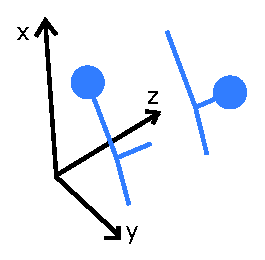
\includegraphics[scale=0.8]{axis.eps}
	\caption{Reference system for the circuit layout.}
	\label{fig:ref_sys}
\end{figure}

\subsection{Layout built with MATLAB}\label{subsec:matlab_layout}
\noindent The following items are optional/mandatory fields of a unique structure.

\begin{description}
\item[magcadImporter \danger] is a variable used to specify whether circuit is described through MATLAB (set to 0) or MagCAD (set to 1).

\item[structure \danger] is a matrix which specify the circuit layout. In each position one can insert a driver, an output, or a molecule. Drivers are identified by the string \textit{Dr}, outputs are identified by the string \textit{out}, molecules are identified by the number of the clock zone to which they belong. 
  
\item[Values\_Dr \danger] is a matrix in which for each driver (row) is specified its input voltage for each time step (column). Must be consistent with \textbf{structure}. 

\item[clockMode] is a variable which specifies which clocking mode to use. The two possible values for this variable are \textcolor{mylilas}{\textquotesingle{phase}\textquotesingle} and \textcolor{mylilas}{\textquotesingle{map}\textquotesingle}. In phase mode, the user MUST include \textbf{stack\_phase}. In map mode, the user MUST include \textbf{ckmap.coords} and \textbf{ckmap.field}. [\textit{default} \textquotesingle{phase}\textquotesingle]

\item[stack\_phase \danger] is a matrix in which for each clock zone (row) is specified the clocking electric field for each time step (column). Must be consistent with \textbf{structure}. 

\item[ckmap.coords \danger] is a matrix which specifies the coordinates in \r{A}ngstr\"{o}m in which the values of the clocking electric field are provided. First column is for z-axis coordinates, second column is for y-axis coordinates. Must be consistent with \textbf{ckmap.field}. 

\item[ckmap.field \danger] is a matrix in which for each coordinates couple (row) specified in \textbf{ckmap.coords} is specified the clocking electric field for each time step (column). Must be consistent with \textbf{ckmap.coords}. 

\item[dist\_z] specifies the intermolecular distance along the z-axis in \r{A}ngstr\"{o}m [\textit{default} 10~\AA]

\item[dist\_y] specifies the intermolecular distance along the y-axis in \r{A}ngstr\"{o}m [\textit{default} 20~\AA~\footnote{In previous versions of SCERPA the default value was \textbf{dist\_z} + inter-dot distance of the bis-ferrocene molecule.}]

\item[molecule] is a char vector containing the name of the molecules, chosen from the \underline{Molecule list} below, even those in brackets [\textit{default} bisfe\_4] 

\item[components] is a matrix, with the same dimensions of the \textbf{structure}, containing in each position the molecule type expressed with the corresponding number in the \underline{Molecule list} below [\textit{default} all elements equal to \textbf{molecule}] \footnote{If \textbf{components} is present, the field \textbf{molecule} is not taken into account. If \textbf{components} is missing, the circuit is composed with the same molecule in each position, and the molecule used is the one specified in the \textbf{molecule} field (default or not).}

\item[rotation\_x] is a matrix with the same dimensions of the \textbf{structure}, containing in each position the molecule rotation around the x-axis expressed in degree [\textit{default} 0\textdegree]

\item[rotation\_y] is a matrix, with the same dimensions of the \textbf{structure}, containing in each position the molecule rotation around the y-axis expressed in degree [\textit{default} 0\textdegree]

\item[rotation\_z] is a matrix, with the same dimensions of the \textbf{structure}, containing in each position the molecule rotation around the z-axis expressed in degree [\textit{default} 0\textdegree]

\item[shift\_x] is a matrix, with the same dimensions of the \textbf{structure}, containing in each position the molecule shift along the x-axis expressed in \r{A}ngstr\"{o}m [\textit{default} 0~\AA]

\item[shift\_y] is a matrix, with the same dimensions of the \textbf{structure}, containing in each position the molecule shift along the y-axis expressed in \r{A}ngstr\"{o}m [\textit{default} 0~\AA]

\item[shift\_z] is a matrix, with the same dimensions of the \textbf{structure}, containing in each position the molecule shift along the z-axis expressed in \r{A}ngstr\"{o}m [\textit{default} 0~\AA]

\item[Vext] is a matrix, with the same dimensions of the \textbf{structure}, containing in each position the fixed external voltage applied onto the molecule expressed in volts [\textit{default} 0~V]

\item[plotLayout] is a variable used to specify whether SCERPA should plot the layout of the circuit (1 is yes, 0 is no) [\textit{default} 0] 

\end{description}


\subsection*{Molecules list}
\noindent Below the list of the available molecules with the identification number used in SCERPA. The terms in brackets specify which molecule is actually associated to the \textit{circuit.molecule} field. 
\begin{itemize}
\item[0 ] $\longrightarrow$  bisfe4\_ox\_counterionOnCarbazole
\item[1 ] $\longrightarrow$  bisfe4\_ox\_counterionOnThiol (bisfe\_4)
\item[2 ] $\longrightarrow$  bisfe4\_ox\_counterionOnThiol\_orca (bisfe\_4\_orca)
\item[3 ] $\longrightarrow$  bisfe4\_ox\_noCounterion
\item[4 ] $\longrightarrow$  bisfe4\_ox\_noCounterion\_TSA\_2states
\item[5 ] $\longrightarrow$  bisfe4\_ox\_noCounterion\_TSA\_3states
\item[6 ] $\longrightarrow$  bisfe4\_sym
\item[7 ] $\longrightarrow$  butane\_ox\_noCounterion (butane)
\item[8 ] $\longrightarrow$  butane\_ox\_noCounterion\_orca
\item[9 ] $\longrightarrow$  butaneCam
\item[10] $\longrightarrow$  decatriene\_ox\_noCounterion (decatriene)
\item[11] $\longrightarrow$  linear\_mol\_w7\_a2000 (linear\_w7)
\item[12] $\longrightarrow$  linear\_mol\_w7\_a3000
\item[13] $\longrightarrow$  linear\_mol\_w9\_a3000 (linear\_w9)
\item[14] $\longrightarrow$  linear\_mol\_w95\_a3000 (linear\_w95)
\end{itemize}

\subsection{Layout built with MagCAD}\label{subsec:magcad_layout}
\noindent The following items are optional/mandatory fields of a unique structure. 

\begin{description}
\item[magcadImporter \danger] is a variable used to specify whether circuit is described through MATLAB (set to 0) or MagCAD (set to 1).

\item[qllFile \danger] contains the path of the \textit{.qll} file in which the circuit under test has been described.

\item[doubleMolDriverMode \danger] is a variable used to specify whether the drivers should be implemented with one molecule (set to 0) or two molecules (set to 1).

\item[Values\_Dr \danger] is a matrix in which for each driver (row) is specified its input voltage for each time step (column). If \textbf{doubleMolDriverMode} is set to 1, in this matrix MUST be present the values for both molecules: the name of the added molecule MUST be the same of the other one followed by \textcolor{mylilas}{\textquotesingle{\_c}\textquotesingle}.

\item[clockMode] is a variable which specifies which clocking mode to use. The two possible values for this variable are \textcolor{mylilas}{\textquotesingle{phase}\textquotesingle} and \textcolor{mylilas}{\textquotesingle{map}\textquotesingle}. In phase mode, the user MUST include \textbf{stack\_phase}. In map mode, the user MUST include \textbf{ckmap.coords} and \textbf{ckmap.field}. [\textit{default} \textquotesingle{phase}\textquotesingle]

\item[stack\_phase \danger] is a matrix in which for each clock zone (row) is specified the clocking electric field for each time step (column).

\item[ckmap.coords \danger] is a matrix which specifies the coordinates in \r{A}ngstr\"{o}m in which the values of the clocking electric field are provided. First column is for z-axis coordinates, second column is for y-axis coordinates. Must be consistent with \textbf{ckmap.field}. 

\item[ckmap.field \danger] is a matrix in which for each coordinates couple (row) specified in \textbf{ckmap.coords} is specified the clocking electric field for each time step (column). Must be consistent with \textbf{ckmap.coords}. 

 
\end{description}


\section{SCERPA settings} \label{sec:settings}
\noindent The following items are optional fields of a unique structure \footnote{Plots settings in this structure refers to runtime plots (they slow down execution).}. 

\begin{description}
%\item[Time definition]: 
%	\begin{itemize}
%	\item \underline{timestep}: [\textit{default} 1]
%	\end{itemize}
%\item[CAD integration]:
%	\begin{itemize}
%	\item \underline{magcadImporter}: set to 1 whether layout is designed with magCAD, 0 otherwise [\textit{default} 0]
%	\item \underline{doubleMolDriverMode}: set to 1 whether the input drivers should be represented with two molecules, 0 otherwise [\textit{default} 0]
%	\end{itemize}

%\item[Energy]:
%	\begin{itemize}
%	\item \underline{energyEval:} set to 1 whether one wants to evaluate the internal energy, the exchange energy, the clock energy, and the total energy. Set to 0 otherwise [\textit{default} 0]
%	\end{itemize}

\item[Algorithm Output and Runtime Plot]:
	\begin{itemize}
	\item \underline{out\_path}: this setting enables the specification of the path for SCERPA output files [\textit{default} \textcolor{mylilas}{\textquotesingle{/scerpaPath/OUTPUT\_FILES}\textquotesingle}] 
	\item \underline{plot\_plotAbsoluteCharge}: if set to 1 it plots the absolute value of the dots charge in the 3D layout plot, otherwise it considers the actual value of the dots charge [\textit{default} 1] 
	\item \underline{plotIntermediateSteps}: if set to 1, it opens a window during the calculation which shows the trend of charges and input voltages at each step of the iterative procedure. Setting to 1 this setting strongly slows down the execution [\textit{default} 0] 
	\item \underline{plotActiveRegionWindow}: if set to 1, during the execution of the code, a figure shows the voltage of all the molecules an highligth the molecules inserted in the Active Region list.  [\textit{default} 0] 
	\item \underline{plot\_3dfig}: if set to 1 it plots the 3D layout of the circuit for each time step [\textit{default} 0] 
	\item \underline{plot\_voltage}: if set to 1 it plots the input voltage on each molecule for each time step [\textit{default} 0] 
	\item \underline{plot\_chargeFig}: if set to 1 it plots the charge value of the logic dots for each molecule, and for each time step [\textit{default} 0] 
%	\item \underline{plot\_logic}: if set to 1, it shows the logical information (0 or 1) propagating in the molecular circuit. The information is evaluated by considering the molecular cell composed by two molecules and using the standard QCA definition  [\textit{default} 0]
	\item \underline{plot\_clock}: if set to 1 it plots the clock field on each molecule for each time step [\textit{default} 0]
	\item \underline{plot\_molnum}: if set to 1, it writes the molecule label in the 3D layout plot [\textit{default} 1] 
	\item \underline{verbosity}: this setting defines how much informations are written in the console during the simulation, if set to 0 means that no data are written, if set to 1 the convergence step is written for each time step, if set to 2 convergence info are written for each time step [\textit{default} 0] 
	\item \underline{pauseStep}: this command, if set to 1, pauses the execution of scerpa at each step of the plotIntermediateSteps='1'. [\textit{default} 0] 
%	\item \underline{fig\_saver}: \textcolor{red}{dà errore} [\textit{default} 'no'] 
	\end{itemize}

\item[Convergence settings]:
	\begin{itemize}
	\item \underline{max\_step}: set the maximum number of SCF iterations, after having reached this value, precision is lowered to LP and then to LLP if needed (see Precision settings below) [\textit{default} 1000] 
	\item \underline{immediateUpdate}: if set to 1, the algorithm updates the charge value onto the dots at each sub-step, one molecule at a time. This let the algorithm to converge faster, but it is far from the physical behaviour, since molecules actually \enquote{update} all together. To speed up the convergence without loosing the physical meaning, one should appropriately choose the damping factor. Hint: set this setting to 0, unless strictly needed [\textit{default} 0] 
	\item \underline{damping}: damping affects the rate and mode of convergence without influencing the final result, if correctly chosen. Value must be in range [0 - 1) [\textit{default} 0.4] 
	\item \underline{autodamping}: if set to 1, it enables the automatic choice of the damping factor based on voltage variation value [\textit{default} 0]
	\end{itemize}
\item[Convergence accelerations]:
	\begin{itemize}
	\item \underline{enableRefining}: if set to 1, once the algorithm reaches convergence it disables the active region and continues the evaluation, it stops otherwise [\textit{default} 1] 
	\item \underline{enableActiveRegion}: if set to 1, the algorithm evaluates the interaction among a reduced set of molecule, avoiding the evaluation of molecules whose charge is not supposed to vary in the current step [\textit{default} 1] 
	\item \underline{activeRegionThreshold}: this value defines which molecules belong to the active region, if the voltage variation is higher  the this value, the molecule is added to the active region list [\textit{default} 0.0015] 
	\item \underline{enableInteractionRadiusMode}: if set to 1, the algorithm evaluate, for each molecule, only the effects of molecules which are close to the one under evaluation (within a specific distance specified by the setting interactionRadius) [\textit{default} 1] 
	\item \underline{interactionRadius}: this value defines the maximum distance (in $\AA$) the algorithm might consider in the evaluation of electric field. Chosen a specific molecule, only the effects generated by the molecule with lower distance than this value will be considered in the evaluation [\textit{default} 101] 
	\end{itemize}
\item[DEBUG informations]:
	\begin{itemize}
	\item \underline{printConvergenceTable}: if set to 1, SCERPA prints the \enquote{Convergence Table}. This table reports all the input voltages of each molecule and the subcomponents related to each intermolecular interaction. It allows detecting possible bugs and errors on SCERPA. [\textit{default} 0] 
	\end{itemize}
\item[Precision]:
	\begin{itemize}
	\item \underline{LPmode}: maximum number of steps to try to reach convergence in Low Precision Mode [\textit{default} 200] 
	\item \underline{LPPmode}: maximum number of steps to try to reach convergence in Very Low Precision Mode [\textit{default} 300] 
	\item \underline{conv\_threshold\_HP}: when the SCF error reaches the convergence threshold, the algorithm stops. If it is not reached, precision is lowered to LP and and the algorithm runs in LPmode. If convergence is not achieved even in this mode, precision is lowered to LLP and and the algorithm runs in LLPmode [\textit{default} 0.000005] 
	\item \underline{conv\_threshold\_LP}: convergence threshold in Low Precision Mode [\textit{default} 0.0005] 
	\item \underline{conv\_threshold\_LLP}: convergence threshold in Very Low Precision Mode [\textit{default} 0.005] 
	\end{itemize}
\item[MATLAB optimization]:
	\begin{itemize}
	\item \underline{enableJit}: if set to 0, the MATLAB just-in-time compiler is disabled. This possibly slows down the calculation, yet allows performing more effective computational complexity analyses [\textit{default 1}] 
	\end{itemize}
\item[Driver saturation]:
	\begin{itemize}
	\item \underline{driverSaturation}: set to 1 whether the charge values of the driver should saturate, 0 otherwise [\textit{default} 0]
	\end{itemize}
\item[Generation of the Additional Information TXT file]:
\begin{itemize}
	\item \underline{dumpClock}: if set to 1, the TXT file reports the clock of each molecule in each timestep [\textit{default} 0]
	\item \underline{dumpVout}: if set to 1, the TXT file reports the voltage of each molecule in each timestep [\textit{default} 0]
	\item \underline{dumpDriver}: if set to 1, the TXT file reports the voltage of each driver in each timestep [\textit{default} 0]
	\item \underline{dumpOutput}: if set to 1, the TXT file reports the voltage of each output in each timestep [\textit{default} 0]
	\item \underline{dumpComputationTime}: if set to 1, the TXT file reports the time duration of each timestep in seconds [\textit{default} 0]
	\item \underline{dumpEnergy}: if set to 1, the TXT file reports energy values in each timestep [\textit{default} 0]
\end{itemize}
\end{description}

\section{SCERPA Viewer settings}\label{sec:viewerSettings}
%There are \underline{two} possible uses of the SCERPA viewer:
%
%\begin{enumerate}
%\item \textbf{Embedded}: the viewer plots the steps of the last SCERPA simulation. Typically, this is used just after a simulation. 
%\item \textbf{On demand}: the viewer plots a single step of a simulation. The viewer requires the layout file (QLL) and the SCERPA results (QSS). This mode is supposed to work with the MagCAD layout only and is not directly compatible with the MATLAB layout generator unless using a porting function (currently used in the embedded mode).
%\end{enumerate}
\noindent The following items are optional fields of a unique structure.

\begin{description}

\item[Output path]:
\begin{itemize}
	\item \underline{out\_path}: MUST be the same path specified for the SCERPA algorithm, where the output files are already present [\textit{default} \textcolor{mylilas}{\textquotesingle{/scerpaPath/OUTPUT\_FILES}\textquotesingle}] 
\end{itemize}

\item[General Plot Settings]:
\begin{itemize}
	\item \underline{fig\_saver}: if set to 1, the viewer saves *.fig files of each picture [\textit{default} 0]
	\item \underline{plotSpan}: the viewer can print a limited number of steps, if plotSpan~=~N, the viewer plots a figure every N steps [\textit{default} 1]
	\item \underline{plotList}: is a vector that can be used to specify which timestep to print (plotList~=~[2 6 7] will print only steps 2, 6 and 7). If set to 0, the viewer plots all the available steps, considering the settings \textbf{plotSpan}. [\textit{default} 0]
\end{itemize}

\item[3D Plot settings]:
\begin{itemize}
	\item \underline{plot\_3dfig}: if set to 1, it enables the 3D plot [\textit{default} 1]
	\item \underline{plot\_3dfig\_plotAbsoluteCharge}: if set to 1, the viewer plots the absolute charge distribution [\textit{default} 1]
	\item \underline{plot\_3dfig\_molnum}: if set to 1, the viewer plots the name of each molecule on the figure [\textit{default} 1]
\end{itemize}

\item[1D Plot settings]:
\begin{itemize}
	\item \underline{plot\_1DCharge}: if set to 1, it enables the 1D plot [\textit{default} 0]
\end{itemize}

\item[Logic Plot settings]:
\begin{itemize}
	\item \underline{plot\_logic}: if set to 1, it enables the logic plot showing the information encoding on the cell according to the standard QCA definition [\textit{default} 0]
\end{itemize}

\item[Potential Plot settings]:
\begin{itemize}
	\item \underline{plot\_potential}: if set to 1, it enables the potential plot showing voltage generated by the molecular charge distribution [\textit{default} 0]
	\item \underline{plot\_potential\_padding}: this value allows enlarging the region where the potential is calculated [\textit{default} 20]
	\item \underline{plot\_potential\_saturationVoltage}: this value enables saturating the potential to improve graphical clarity [\textit{default} 6]
	\item \underline{plot\_potential\_tipHeight}: this value, in $\AA$, defines the height of the virtual tip measuring the potential [\textit{default} -5.5]
\end{itemize}

\item[Waveform Plot settings]:
\begin{itemize}
	\item \underline{plot\_waveform}: if set to 1, it enables the plot of input/output waveform (Warning: this plot requires input/output information in the Additional Information file. Be sure the simulation was run with \textbf{dumpDriver}~=~1 and \textbf{dumpOutput}~=~1) [\textit{default} 0]	
\end{itemize}


\end{description}

\section{Examples}
\subsection{Three phase wire}
\lstinputlisting{threePhasesWire.m}

\subsection{Three phase wire clock map}
\lstinputlisting{threePasesWireClockMap.m}

\newpage
\subsection{Three phase wire multi-molecule}
\lstinputlisting{threePhasesWireMultiMol.m}

\section{SCERPA Bibliography}\label{sec:biblio}

\begin{itemize}
	\item Y. Ardesi, G. Turvani, M. Graziano and G. Piccinini, "SCERPA Simulation of Clocked Molecular Field-Coupling Nanocomputing," in IEEE Transactions on Very Large Scale Integration (VLSI) Systems, vol. 29, no. 3, pp. 558-567, March 2021, doi: 10.1109/TVLSI.2020.3045198.
	\item Y. Ardesi, R. Wang, G. Turvani, G. Piccinini and M. Graziano, "SCERPA: A Self-Consistent Algorithm for the Evaluation of the Information Propagation in Molecular Field-Coupled Nanocomputing," in IEEE Transactions on Computer-Aided Design of Integrated Circuits and Systems, vol. 39, no. 10, pp. 2749-2760, Oct. 2020, doi: 10.1109/TCAD.2019.2960360.
	\item R. Wang, M. Chilla, A. Palucci, M. Graziano and G. Piccinini, "An effective algorithm for clocked field-coupled nanocomputing paradigm," 2016 IEEE Nanotechnology Materials and Devices Conference (NMDC), 2016, pp. 1-2, doi: 10.1109/NMDC.2016.7777166.
\end{itemize}


\end{document}